% Options for packages loaded elsewhere
% Options for packages loaded elsewhere
\PassOptionsToPackage{unicode}{hyperref}
\PassOptionsToPackage{hyphens}{url}
%
\documentclass[
  english,
  russian,
  12pt,
  a4paper,
  DIV=11,
  numbers=noendperiod]{scrreprt}
\usepackage{xcolor}
\usepackage{amsmath,amssymb}
\setcounter{secnumdepth}{5}
\usepackage{iftex}
\ifPDFTeX
  \usepackage[T1]{fontenc}
  \usepackage[utf8]{inputenc}
  \usepackage{textcomp} % provide euro and other symbols
\else % if luatex or xetex
  \usepackage{unicode-math} % this also loads fontspec
  \defaultfontfeatures{Scale=MatchLowercase}
  \defaultfontfeatures[\rmfamily]{Ligatures=TeX,Scale=1}
\fi
\usepackage{lmodern}
\ifPDFTeX\else
  % xetex/luatex font selection
  \setmainfont[Ligatures=Common,Ligatures=TeX,Scale=0.94]{IBM Plex
Serif}
  \setsansfont[Ligatures=Common,Ligatures=TeX,Scale=MatchLowercase,Scale=0.94]{IBM
Plex Sans}
  \setmonofont[Scale=MatchLowercase,Scale=0.94]{DejaVu Sans Mono}
  \setmathfont[]{STIX Two Math}
\fi
% Use upquote if available, for straight quotes in verbatim environments
\IfFileExists{upquote.sty}{\usepackage{upquote}}{}
\IfFileExists{microtype.sty}{% use microtype if available
  \usepackage[]{microtype}
  \UseMicrotypeSet[protrusion]{basicmath} % disable protrusion for tt fonts
}{}
\usepackage{setspace}
% Make \paragraph and \subparagraph free-standing
\makeatletter
\ifx\paragraph\undefined\else
  \let\oldparagraph\paragraph
  \renewcommand{\paragraph}{
    \@ifstar
      \xxxParagraphStar
      \xxxParagraphNoStar
  }
  \newcommand{\xxxParagraphStar}[1]{\oldparagraph*{#1}\mbox{}}
  \newcommand{\xxxParagraphNoStar}[1]{\oldparagraph{#1}\mbox{}}
\fi
\ifx\subparagraph\undefined\else
  \let\oldsubparagraph\subparagraph
  \renewcommand{\subparagraph}{
    \@ifstar
      \xxxSubParagraphStar
      \xxxSubParagraphNoStar
  }
  \newcommand{\xxxSubParagraphStar}[1]{\oldsubparagraph*{#1}\mbox{}}
  \newcommand{\xxxSubParagraphNoStar}[1]{\oldsubparagraph{#1}\mbox{}}
\fi
\makeatother

\usepackage{color}
\usepackage{fancyvrb}
\newcommand{\VerbBar}{|}
\newcommand{\VERB}{\Verb[commandchars=\\\{\}]}
\DefineVerbatimEnvironment{Highlighting}{Verbatim}{commandchars=\\\{\}}
% Add ',fontsize=\small' for more characters per line
\usepackage{framed}
\definecolor{shadecolor}{RGB}{241,243,245}
\newenvironment{Shaded}{\begin{snugshade}}{\end{snugshade}}
\newcommand{\AlertTok}[1]{\textcolor[rgb]{0.68,0.00,0.00}{#1}}
\newcommand{\AnnotationTok}[1]{\textcolor[rgb]{0.37,0.37,0.37}{#1}}
\newcommand{\AttributeTok}[1]{\textcolor[rgb]{0.40,0.45,0.13}{#1}}
\newcommand{\BaseNTok}[1]{\textcolor[rgb]{0.68,0.00,0.00}{#1}}
\newcommand{\BuiltInTok}[1]{\textcolor[rgb]{0.00,0.23,0.31}{#1}}
\newcommand{\CharTok}[1]{\textcolor[rgb]{0.13,0.47,0.30}{#1}}
\newcommand{\CommentTok}[1]{\textcolor[rgb]{0.37,0.37,0.37}{#1}}
\newcommand{\CommentVarTok}[1]{\textcolor[rgb]{0.37,0.37,0.37}{\textit{#1}}}
\newcommand{\ConstantTok}[1]{\textcolor[rgb]{0.56,0.35,0.01}{#1}}
\newcommand{\ControlFlowTok}[1]{\textcolor[rgb]{0.00,0.23,0.31}{\textbf{#1}}}
\newcommand{\DataTypeTok}[1]{\textcolor[rgb]{0.68,0.00,0.00}{#1}}
\newcommand{\DecValTok}[1]{\textcolor[rgb]{0.68,0.00,0.00}{#1}}
\newcommand{\DocumentationTok}[1]{\textcolor[rgb]{0.37,0.37,0.37}{\textit{#1}}}
\newcommand{\ErrorTok}[1]{\textcolor[rgb]{0.68,0.00,0.00}{#1}}
\newcommand{\ExtensionTok}[1]{\textcolor[rgb]{0.00,0.23,0.31}{#1}}
\newcommand{\FloatTok}[1]{\textcolor[rgb]{0.68,0.00,0.00}{#1}}
\newcommand{\FunctionTok}[1]{\textcolor[rgb]{0.28,0.35,0.67}{#1}}
\newcommand{\ImportTok}[1]{\textcolor[rgb]{0.00,0.46,0.62}{#1}}
\newcommand{\InformationTok}[1]{\textcolor[rgb]{0.37,0.37,0.37}{#1}}
\newcommand{\KeywordTok}[1]{\textcolor[rgb]{0.00,0.23,0.31}{\textbf{#1}}}
\newcommand{\NormalTok}[1]{\textcolor[rgb]{0.00,0.23,0.31}{#1}}
\newcommand{\OperatorTok}[1]{\textcolor[rgb]{0.37,0.37,0.37}{#1}}
\newcommand{\OtherTok}[1]{\textcolor[rgb]{0.00,0.23,0.31}{#1}}
\newcommand{\PreprocessorTok}[1]{\textcolor[rgb]{0.68,0.00,0.00}{#1}}
\newcommand{\RegionMarkerTok}[1]{\textcolor[rgb]{0.00,0.23,0.31}{#1}}
\newcommand{\SpecialCharTok}[1]{\textcolor[rgb]{0.37,0.37,0.37}{#1}}
\newcommand{\SpecialStringTok}[1]{\textcolor[rgb]{0.13,0.47,0.30}{#1}}
\newcommand{\StringTok}[1]{\textcolor[rgb]{0.13,0.47,0.30}{#1}}
\newcommand{\VariableTok}[1]{\textcolor[rgb]{0.07,0.07,0.07}{#1}}
\newcommand{\VerbatimStringTok}[1]{\textcolor[rgb]{0.13,0.47,0.30}{#1}}
\newcommand{\WarningTok}[1]{\textcolor[rgb]{0.37,0.37,0.37}{\textit{#1}}}

\usepackage{longtable,booktabs,array}
\newcounter{none} % for unnumbered tables
\usepackage{calc} % for calculating minipage widths
% Correct order of tables after \paragraph or \subparagraph
\usepackage{etoolbox}
\makeatletter
\patchcmd\longtable{\par}{\if@noskipsec\mbox{}\fi\par}{}{}
\makeatother
% Allow footnotes in longtable head/foot
\IfFileExists{footnotehyper.sty}{\usepackage{footnotehyper}}{\usepackage{footnote}}
\makesavenoteenv{longtable}
\usepackage{graphicx}
\makeatletter
\newsavebox\pandoc@box
\newcommand*\pandocbounded[1]{% scales image to fit in text height/width
  \sbox\pandoc@box{#1}%
  \Gscale@div\@tempa{\textheight}{\dimexpr\ht\pandoc@box+\dp\pandoc@box\relax}%
  \Gscale@div\@tempb{\linewidth}{\wd\pandoc@box}%
  \ifdim\@tempb\p@<\@tempa\p@\let\@tempa\@tempb\fi% select the smaller of both
  \ifdim\@tempa\p@<\p@\scalebox{\@tempa}{\usebox\pandoc@box}%
  \else\usebox{\pandoc@box}%
  \fi%
}
% Set default figure placement to htbp
\def\fps@figure{htbp}
\makeatother



\ifLuaTeX
\usepackage[bidi=basic,shorthands=off,provide=*]{babel}
\else
\usepackage[bidi=default,shorthands=off,provide=*]{babel}
\fi
\ifPDFTeX
\else
\babelfont{rm}[Ligatures=Common,Ligatures=TeX,Scale=0.94]{IBM Plex
Serif}
\fi
\ifLuaTeX
  \usepackage{selnolig} % disable illegal ligatures
\fi


\setlength{\emergencystretch}{3em} % prevent overfull lines

\providecommand{\tightlist}{%
  \setlength{\itemsep}{0pt}\setlength{\parskip}{0pt}}



 
\usepackage[style=gost-numeric,backend=biber,langhook=extras,autolang=other*]{biblatex}
\addbibresource{bib/cite.bib}

\usepackage[]{csquotes}

\usepackage{indentfirst}
\usepackage{float}
\floatplacement{figure}{H}

% \IfFileExists{plex-otf.sty}{
%   \usepackage[
%     RM={Scale=0.94},SS={Scale=0.94},SScon={Scale=0.94},TT={Scale=MatchLowercase,FakeStretch=0.9},
%     DefaultFeatures={Ligatures=Common}
%   ]{plex-otf}
% }{
%   \usepackage{libertine}
% }
\KOMAoption{captions}{tableheading}
\makeatletter
\@ifpackageloaded{caption}{}{\usepackage{caption}}
\AtBeginDocument{%
\ifdefined\contentsname
  \renewcommand*\contentsname{Содержание}
\else
  \newcommand\contentsname{Содержание}
\fi
\ifdefined\listfigurename
  \renewcommand*\listfigurename{Список иллюстраций}
\else
  \newcommand\listfigurename{Список иллюстраций}
\fi
\ifdefined\listtablename
  \renewcommand*\listtablename{Список таблиц}
\else
  \newcommand\listtablename{Список таблиц}
\fi
\ifdefined\figurename
  \renewcommand*\figurename{Рисунок}
\else
  \newcommand\figurename{Рисунок}
\fi
\ifdefined\tablename
  \renewcommand*\tablename{Таблица}
\else
  \newcommand\tablename{Таблица}
\fi
}
\@ifpackageloaded{float}{}{\usepackage{float}}
\floatstyle{ruled}
\@ifundefined{c@chapter}{\newfloat{codelisting}{h}{lop}}{\newfloat{codelisting}{h}{lop}[chapter]}
\floatname{codelisting}{Список}
\newcommand*\listoflistings{\listof{codelisting}{Листинги}}
\makeatother
\makeatletter
\makeatother
\makeatletter
\@ifpackageloaded{caption}{}{\usepackage{caption}}
\@ifpackageloaded{subcaption}{}{\usepackage{subcaption}}
\makeatother
\usepackage{bookmark}
\IfFileExists{xurl.sty}{\usepackage{xurl}}{} % add URL line breaks if available
\urlstyle{same}
% fallback for those not using the hyperref driver hyperxmp:
\makeatletter
\@ifundefined{xmpquote}{\newcommand{\xmpquote}[1]{#1}}{}
\makeatother
\hypersetup{
  pdftitle={Лабораторная работа №4. Работа с программными пакетами},
  pdfauthor={Мацюк Константин Владимирович},
  pdflang={ru-RU},
  hidelinks,
  pdfcreator={LaTeX via pandoc}}


\title{Лабораторная работа №4. Работа с программными пакетами}
\usepackage{etoolbox}
\makeatletter
\providecommand{\subtitle}[1]{% add subtitle to \maketitle
  \apptocmd{\@title}{\par {\large #1 \par}}{}{}
}
\makeatother
\subtitle{Дисциплина: Основы администрирования операционных систем}
\author{Мацюк Константин Владимирович}
\date{}
\begin{document}
\maketitle

\renewcommand*\contentsname{Содержание}
{
\setcounter{tocdepth}{1}
\tableofcontents
}
\listoffigures
\listoftables

\setstretch{1.5}
\chapter{Цель
работы}\label{ux446ux435ux43bux44c-ux440ux430ux431ux43eux442ux44b}

Получить навыки работы с репозиториями и менеджерами пакетов.

\chapter{Задание}\label{ux437ux430ux434ux430ux43dux438ux435}

\begin{enumerate}
\def\labelenumi{\arabic{enumi}.}
\tightlist
\item
  Изучить, как и в каких файлах подключаются репозитории для установки
  программного обеспечения; изучить основные возможности (поиск,
  установка, обновление, удаление пакета, работа с историей действий)
  команды \texttt{dnf} (см. раздел 4.4.1).
\item
  Изучить и повторить процесс установки/удаления определённого пакета с
  использованием возможностей \texttt{dnf} (см. раздел 4.4.1).
\item
  Изучить и повторить процесс установки/удаления определённого пакета с
  использованием возможностей \texttt{rpm} (см. раздел 4.4.2).
\end{enumerate}

\chapter{Теоретическое
введение}\label{ux442ux435ux43eux440ux435ux442ux438ux447ux435ux441ux43aux43eux435-ux432ux432ux435ux434ux435ux43dux438ux435}

Пакетный менеджер \texttt{dnf} используется в популярных
Linux-дистрибутивах для установки, удаления и других действий с
пакетами. Основные команды \texttt{dnf} приведены в методическом пособии
(раздел 4.2.1). Опции \texttt{dnf} описаны в разделе 4.2.2. Расширение
возможностей \texttt{dnf} достигается установкой пакета
\texttt{yum-utils} (раздел 4.2.3). Конфигурационные файлы \texttt{dnf} и
их расположение описаны в разделе 4.2.4, некоторые опции
\texttt{dnf.conf} --- в разделе 4.2.5, полезные плагины --- в разделе
4.2.6, работа через прокси-сервер --- в разделе 4.2.7.

В табл.~\ref{tbl-dnf-files} приведено краткое описание основных
конфигурационных файлов и каталогов \texttt{dnf}.

\begin{longtable}[]{@{}
  >{\raggedright\arraybackslash}p{(\linewidth - 2\tabcolsep) * \real{0.2358}}
  >{\raggedright\arraybackslash}p{(\linewidth - 2\tabcolsep) * \real{0.7642}}@{}}
\caption{Основные конфигурационные файлы и каталоги
dnf}\label{tbl-dnf-files}\tabularnewline
\toprule\noalign{}
\begin{minipage}[b]{\linewidth}\raggedright
Файл/каталог
\end{minipage} & \begin{minipage}[b]{\linewidth}\raggedright
Описание
\end{minipage} \\
\midrule\noalign{}
\endfirsthead
\toprule\noalign{}
\begin{minipage}[b]{\linewidth}\raggedright
Файл/каталог
\end{minipage} & \begin{minipage}[b]{\linewidth}\raggedright
Описание
\end{minipage} \\
\midrule\noalign{}
\endhead
\bottomrule\noalign{}
\endlastfoot
\texttt{/etc/dnf/dnf.conf} & Основной конфигурационный файл
\texttt{dnf} \\
\texttt{/etc/dnf/} & Директория с конфигурациями (например,
dnf-плагины) \\
\texttt{/etc/yum.repos.d/} & Директория с информацией о репозиториях \\
\texttt{/var/cache/dnf/} & Директория, где \texttt{dnf} хранит кэш и
файлы базы (по умолчанию) \\
\texttt{/var/log/dnf.log} & Лог-файл выполнения транзакций (по
умолчанию) \\
\end{longtable}

\chapter{Выполнение лабораторной
работы}\label{ux432ux44bux43fux43eux43bux43dux435ux43dux438ux435-ux43bux430ux431ux43eux440ux430ux442ux43eux440ux43dux43eux439-ux440ux430ux431ux43eux442ux44b}

\section{Работа с
репозиториями}\label{ux440ux430ux431ux43eux442ux430-ux441-ux440ux435ux43fux43eux437ux438ux442ux43eux440ux438ux44fux43cux438}

В консоли перешёл в режим работы суперпользователя, выполнив команду
\texttt{su\ -} (рис.~\ref{fig-001}).

\begin{figure}

\centering{

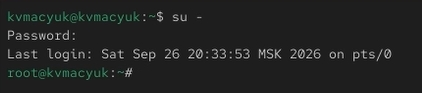
\includegraphics[width=0.7\linewidth,height=\textheight,keepaspectratio]{image/1.jpg}

}

\caption{\label{fig-001}Получение прав root}

\end{figure}%

Перешёл в каталог \texttt{/etc/yum.repos.d} и изучил содержание каталога
и файлов репозиториев (рис.~\ref{fig-002}).

\begin{figure}

\centering{

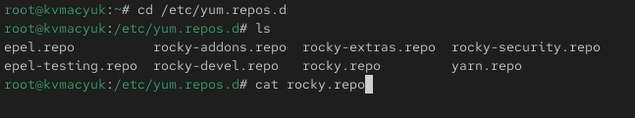
\includegraphics[width=0.7\linewidth,height=\textheight,keepaspectratio]{image/2.jpg}

}

\caption{\label{fig-002}Переход в каталог репозиториев}

\end{figure}%

Вывел на экран список репозиториев командой \texttt{dnf\ repolist}
(рис.~\ref{fig-003}). Полученная информация показывает подключённые
репозитории: appstream, baseos, epel, extras, yarn.

\begin{figure}

\centering{

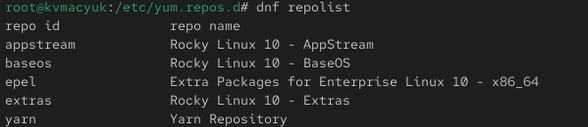
\includegraphics[width=0.7\linewidth,height=\textheight,keepaspectratio]{image/3.jpg}

}

\caption{\label{fig-003}Просмотр списка активных репозиториев}

\end{figure}%

Вывел на экран список пакетов, в названии или описании которых есть
слово \texttt{user}, командой \texttt{dnf\ search\ user}
(рис.~\ref{fig-004}, рис.~\ref{fig-005}).

\begin{figure}

\centering{

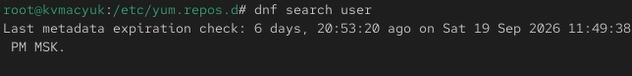
\includegraphics[width=0.7\linewidth,height=\textheight,keepaspectratio]{image/4.jpg}

}

\caption{\label{fig-004}Поиск пакета (начало)}

\end{figure}%

\begin{figure}

\centering{

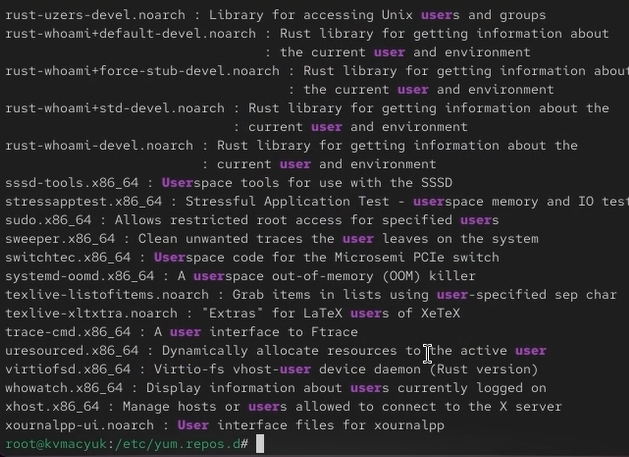
\includegraphics[width=0.7\linewidth,height=\textheight,keepaspectratio]{image/5.jpg}

}

\caption{\label{fig-005}Результаты поиска}

\end{figure}%

Установил \texttt{nmap}, предварительно изучив информацию по имеющимся
пакетам (рис.~\ref{fig-006}---рис.~\ref{fig-010}).

\begin{Shaded}
\begin{Highlighting}[]
\ExtensionTok{dnf}\NormalTok{ search nmap}
\ExtensionTok{dnf}\NormalTok{ info nmap}
\ExtensionTok{dnf}\NormalTok{ install nmap}
\ExtensionTok{dnf}\NormalTok{ install nmap}\DataTypeTok{\textbackslash{}*}
\end{Highlighting}
\end{Shaded}

\begin{figure}

\centering{

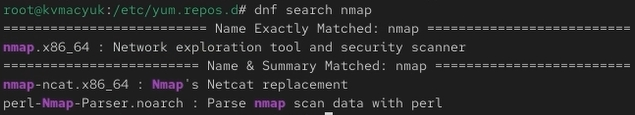
\includegraphics[width=0.7\linewidth,height=\textheight,keepaspectratio]{image/6.jpg}

}

\caption{\label{fig-006}Поиск пакета nmap}

\end{figure}%

\begin{figure}

\centering{

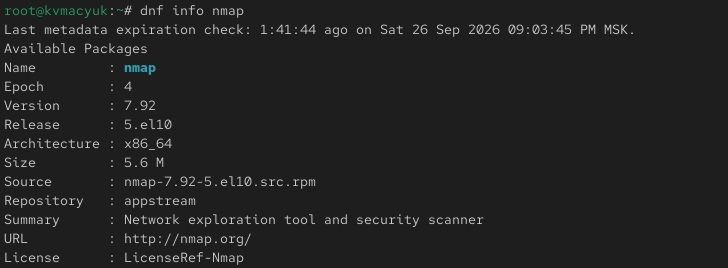
\includegraphics[width=0.7\linewidth,height=\textheight,keepaspectratio]{image/7.jpg}

}

\caption{\label{fig-007}Информация о пакете (начало)}

\end{figure}%

\begin{figure}

\centering{

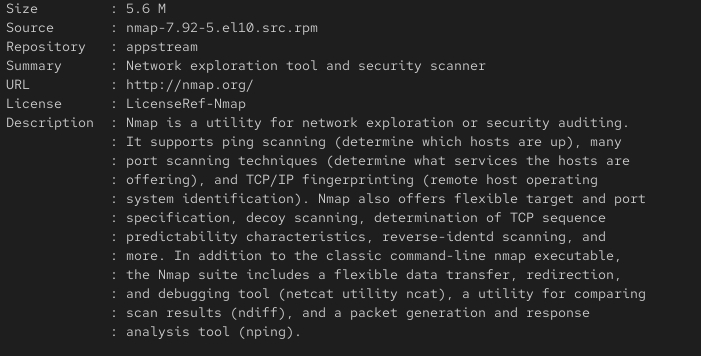
\includegraphics[width=0.7\linewidth,height=\textheight,keepaspectratio]{image/8.jpg}

}

\caption{\label{fig-008}Информация о пакете (продолжение)}

\end{figure}%

\begin{figure}

\centering{

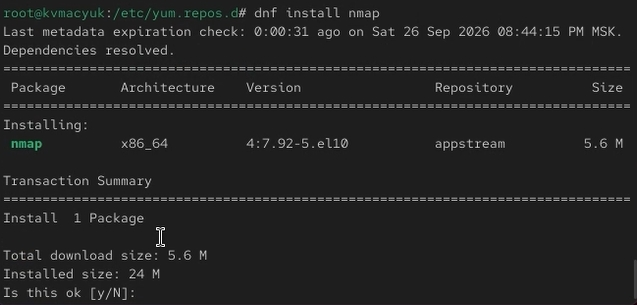
\includegraphics[width=0.7\linewidth,height=\textheight,keepaspectratio]{image/9.jpg}

}

\caption{\label{fig-009}Установка nmap}

\end{figure}%

\begin{figure}

\centering{

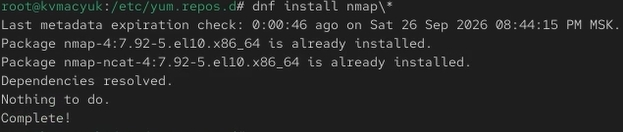
\includegraphics[width=0.7\linewidth,height=\textheight,keepaspectratio]{image/10.jpg}

}

\caption{\label{fig-010}Установка nmap*}

\end{figure}%

Разница между \texttt{dnf\ install\ nmap} и
\texttt{dnf\ install\ nmap*}: первая команда устанавливает только пакет
\texttt{nmap}, вторая --- все пакеты, имя которых начинается с
\texttt{nmap} (например, \texttt{nmap-ncat}). В моем случае все пакеты,
имя которых начинается с \texttt{nmap} уже установлены

Удалил \texttt{nmap} (рис.~\ref{fig-011}, рис.~\ref{fig-012}).

\begin{Shaded}
\begin{Highlighting}[]
\ExtensionTok{dnf}\NormalTok{ remove nmap}
\ExtensionTok{dnf}\NormalTok{ remove nmap}\DataTypeTok{\textbackslash{}*}
\end{Highlighting}
\end{Shaded}

\begin{figure}

\centering{

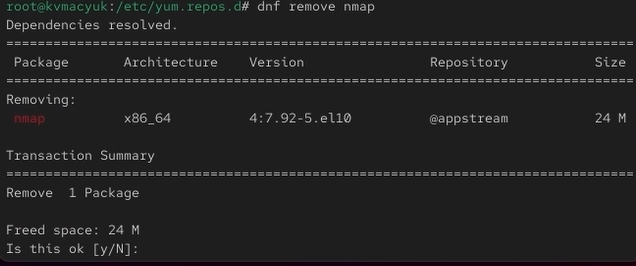
\includegraphics[width=0.7\linewidth,height=\textheight,keepaspectratio]{image/11.jpg}

}

\caption{\label{fig-011}Удаление пакета nmap}

\end{figure}%

\begin{figure}

\centering{

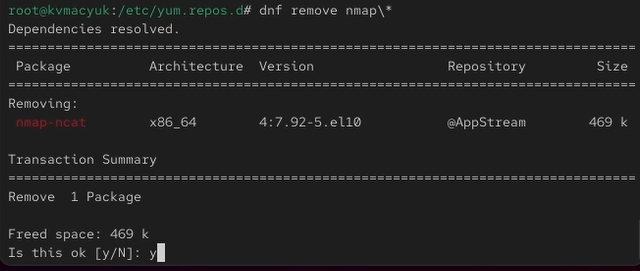
\includegraphics[width=0.7\linewidth,height=\textheight,keepaspectratio]{image/12.jpg}

}

\caption{\label{fig-012}Удаление сопутствующих пакетов}

\end{figure}%

Получил список имеющихся групп пакетов, затем установил группу пакетов
RPM Development Tools (рис.~\ref{fig-013}---рис.~\ref{fig-016}).

\begin{Shaded}
\begin{Highlighting}[]
\ExtensionTok{dnf}\NormalTok{ groups list}
\VariableTok{LANG}\OperatorTok{=}\NormalTok{C }\ExtensionTok{dnf}\NormalTok{ groups list}
\ExtensionTok{dnf}\NormalTok{ groups info }\StringTok{"RPM Development Tools"}
\ExtensionTok{dnf}\NormalTok{ groupinstall }\StringTok{"RPM Development Tools"}
\end{Highlighting}
\end{Shaded}

\begin{figure}

\centering{

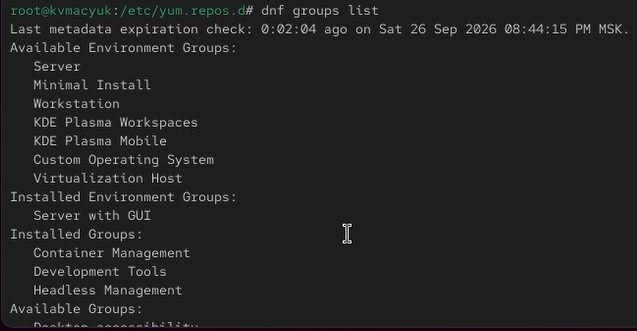
\includegraphics[width=0.7\linewidth,height=\textheight,keepaspectratio]{image/13.jpg}

}

\caption{\label{fig-013}Список групп пакетов}

\end{figure}%

\begin{figure}

\centering{

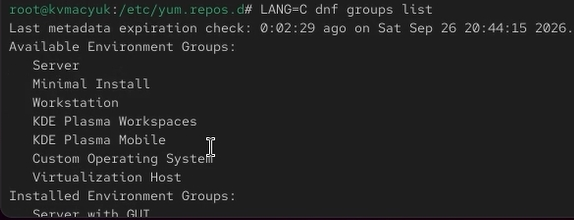
\includegraphics[width=0.7\linewidth,height=\textheight,keepaspectratio]{image/14.jpg}

}

\caption{\label{fig-014}Список групп с локализацией}

\end{figure}%

\begin{figure}

\centering{

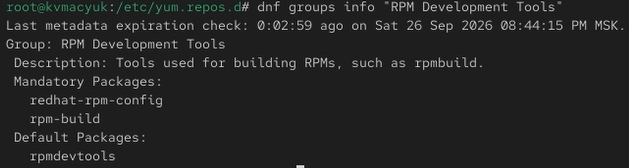
\includegraphics[width=0.7\linewidth,height=\textheight,keepaspectratio]{image/15.jpg}

}

\caption{\label{fig-015}Информация о группе RPM Development Tools}

\end{figure}%

\begin{figure}

\centering{

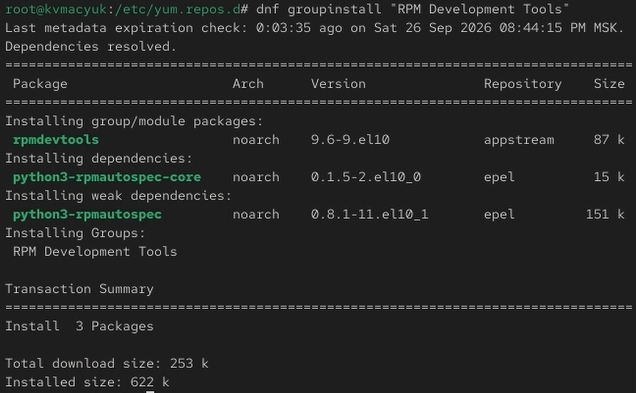
\includegraphics[width=0.7\linewidth,height=\textheight,keepaspectratio]{image/16.jpg}

}

\caption{\label{fig-016}Установка группы RPM Development Tools}

\end{figure}%

Для удаления группы пакетов RPM Development Tools воспользовался
командой \texttt{dnf\ groupremove\ "RPM\ Development\ Tools"}
(рис.~\ref{fig-017}).

\begin{figure}

\centering{

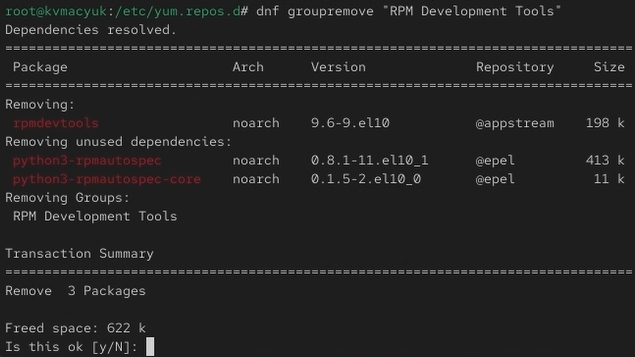
\includegraphics[width=0.7\linewidth,height=\textheight,keepaspectratio]{image/17.jpg}

}

\caption{\label{fig-017}Удаление группы RPM Development Tools}

\end{figure}%

Посмотрел историю использования команды \texttt{dnf} и отменил последнее
действие (рис.~\ref{fig-018}, рис.~\ref{fig-019}).

\begin{Shaded}
\begin{Highlighting}[]
\ExtensionTok{dnf}\NormalTok{ history}
\ExtensionTok{dnf}\NormalTok{ history undo 13}
\end{Highlighting}
\end{Shaded}

\begin{figure}

\centering{

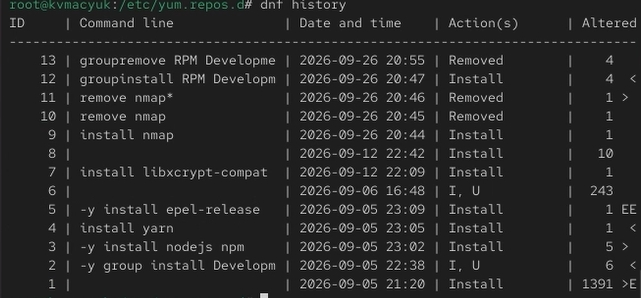
\includegraphics[width=0.7\linewidth,height=\textheight,keepaspectratio]{image/18.jpg}

}

\caption{\label{fig-018}История транзакций dnf}

\end{figure}%

\begin{figure}

\centering{

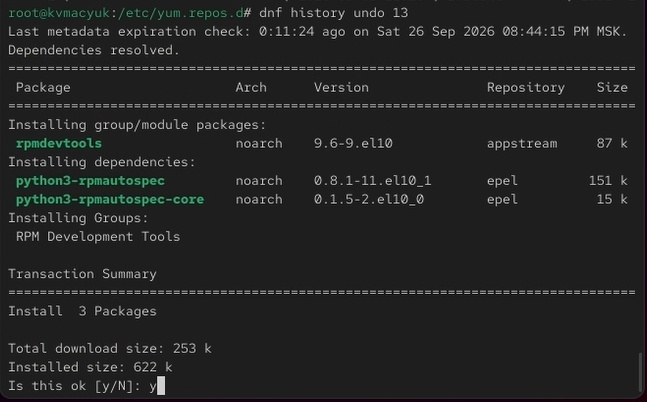
\includegraphics[width=0.7\linewidth,height=\textheight,keepaspectratio]{image/19.jpg}

}

\caption{\label{fig-019}Отмена транзакции (undo)}

\end{figure}%

\section{Использование
rpm}\label{ux438ux441ux43fux43eux43bux44cux437ux43eux432ux430ux43dux438ux435-rpm}

Предположим, что требуется установить текстовый браузер \texttt{lynx} из
rpm-пакета.

Скачал rpm-пакет \texttt{lynx} (рис.~\ref{fig-020}, рис.~\ref{fig-021}).

\begin{Shaded}
\begin{Highlighting}[]
\ExtensionTok{dnf}\NormalTok{ list lynx}
\ExtensionTok{dnf}\NormalTok{ install lynx }\AttributeTok{{-}{-}downloadonly}
\end{Highlighting}
\end{Shaded}

\begin{figure}

\centering{

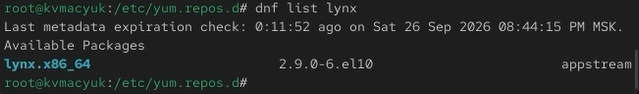
\includegraphics[width=0.7\linewidth,height=\textheight,keepaspectratio]{image/20.jpg}

}

\caption{\label{fig-020}Поиск пакета lynx}

\end{figure}%

\begin{figure}

\centering{

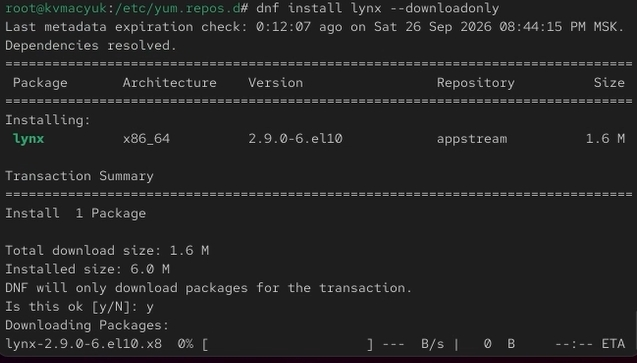
\includegraphics[width=0.7\linewidth,height=\textheight,keepaspectratio]{image/21.jpg}

}

\caption{\label{fig-021}Скачивание пакета без установки}

\end{figure}%

Нашёл каталог, в который был помещён пакет после загрузки
(рис.~\ref{fig-022}).

\begin{Shaded}
\begin{Highlighting}[]
\FunctionTok{find}\NormalTok{ /var/cache/dnf/ }\AttributeTok{{-}name}\NormalTok{ lynx}\PreprocessorTok{*}
\end{Highlighting}
\end{Shaded}

\begin{figure}

\centering{

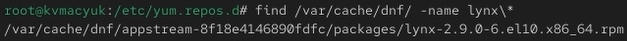
\includegraphics[width=0.7\linewidth,height=\textheight,keepaspectratio]{image/22.jpg}

}

\caption{\label{fig-022}Поиск скачанного файла}

\end{figure}%

Перешёл в этот каталог и затем установил rpm-пакет (рис.~\ref{fig-023}).

\begin{Shaded}
\begin{Highlighting}[]
\ExtensionTok{rpm} \AttributeTok{{-}Uhv}\NormalTok{ lynx{-}}\OperatorTok{\textless{}}\NormalTok{версия}\OperatorTok{\textgreater{}}\NormalTok{.rpm}
\end{Highlighting}
\end{Shaded}

\begin{figure}

\centering{

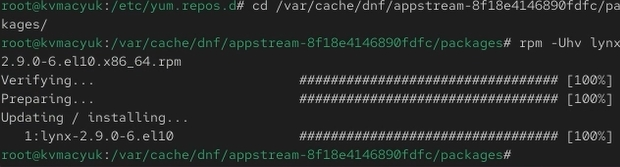
\includegraphics[width=0.7\linewidth,height=\textheight,keepaspectratio]{image/23.jpg}

}

\caption{\label{fig-023}Ручная установка через rpm}

\end{figure}%

Определил расположение исполняемого файла (рис.~\ref{fig-024}).

\begin{Shaded}
\begin{Highlighting}[]
\FunctionTok{which}\NormalTok{ lynx}
\end{Highlighting}
\end{Shaded}

\begin{figure}

\centering{

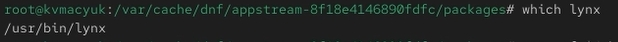
\includegraphics[width=0.7\linewidth,height=\textheight,keepaspectratio]{image/24.jpg}

}

\caption{\label{fig-024}Проверка пути установки}

\end{figure}%

Используя \texttt{rpm}, определил по имени файла, к какому пакету
принадлежит \texttt{lynx}, и получил дополнительную информацию о
содержимом пакета (рис.~\ref{fig-025}, рис.~\ref{fig-026}).

\begin{Shaded}
\begin{Highlighting}[]
\ExtensionTok{rpm} \AttributeTok{{-}qf} \VariableTok{$(}\FunctionTok{which}\NormalTok{ lynx}\VariableTok{)}
\ExtensionTok{rpm} \AttributeTok{{-}qi}\NormalTok{ lynx}
\end{Highlighting}
\end{Shaded}

\begin{figure}

\centering{

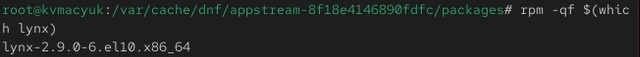
\includegraphics[width=0.7\linewidth,height=\textheight,keepaspectratio]{image/25.jpg}

}

\caption{\label{fig-025}Определение пакета по файлу}

\end{figure}%

\begin{figure}

\centering{

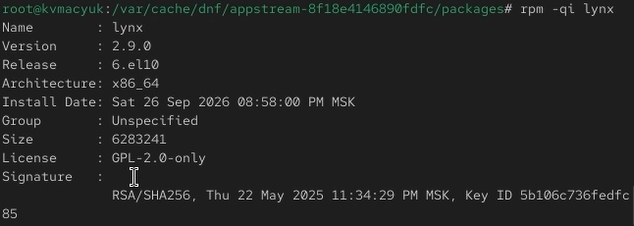
\includegraphics[width=0.7\linewidth,height=\textheight,keepaspectratio]{image/26.jpg}

}

\caption{\label{fig-026}Детальная информация о пакете}

\end{figure}%

Получил список всех файлов в пакете, а также вывел перечень файлов с
документацией пакета (рис.~\ref{fig-027}---рис.~\ref{fig-030}).
Посмотрел файлы документации, применив команду \texttt{man\ lynx}.

\begin{Shaded}
\begin{Highlighting}[]
\ExtensionTok{rpm} \AttributeTok{{-}ql}\NormalTok{ lynx}
\ExtensionTok{rpm} \AttributeTok{{-}qd}\NormalTok{ lynx}
\FunctionTok{man}\NormalTok{ lynx}
\end{Highlighting}
\end{Shaded}

\begin{figure}

\centering{

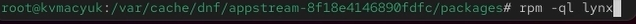
\includegraphics[width=0.7\linewidth,height=\textheight,keepaspectratio]{image/27.jpg}

}

\caption{\label{fig-027}Список файлов пакета (начало)}

\end{figure}%

\begin{figure}

\centering{

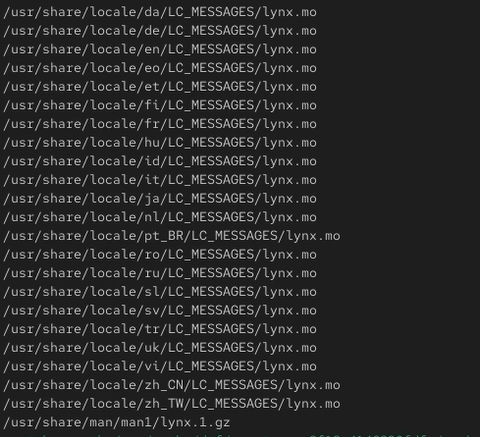
\includegraphics[width=0.7\linewidth,height=\textheight,keepaspectratio]{image/28.jpg}

}

\caption{\label{fig-028}Список файлов пакета (продолжение)}

\end{figure}%

\begin{figure}

\centering{

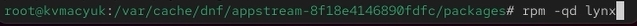
\includegraphics[width=0.7\linewidth,height=\textheight,keepaspectratio]{image/29.jpg}

}

\caption{\label{fig-029}Список документации (запрос)}

\end{figure}%

\begin{figure}

\centering{

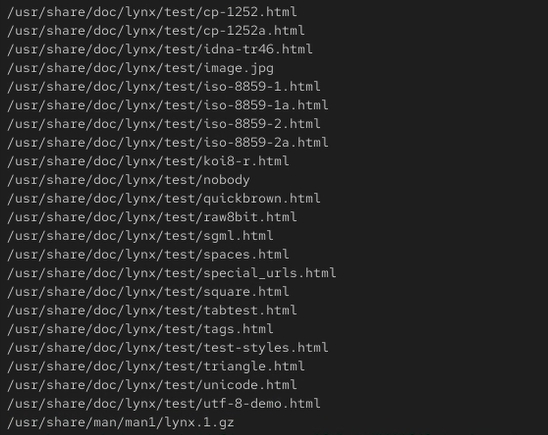
\includegraphics[width=0.7\linewidth,height=\textheight,keepaspectratio]{image/30.jpg}

}

\caption{\label{fig-030}Список документации (вывод)}

\end{figure}%

\begin{figure}

\centering{

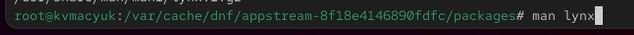
\includegraphics[width=0.7\linewidth,height=\textheight,keepaspectratio]{image/31.jpg}

}

\caption{\label{fig-031}Просмотр справки man}

\end{figure}%

Вывел на экран перечень и месторасположение конфигурационных файлов
пакета (рис.~\ref{fig-032}).

\begin{Shaded}
\begin{Highlighting}[]
\ExtensionTok{rpm} \AttributeTok{{-}qc}\NormalTok{ lynx}
\end{Highlighting}
\end{Shaded}

\begin{figure}

\centering{

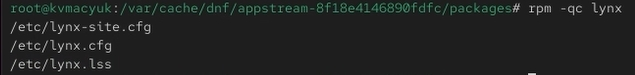
\includegraphics[width=0.7\linewidth,height=\textheight,keepaspectratio]{image/32.jpg}

}

\caption{\label{fig-032}Поиск конфигурационных файлов}

\end{figure}%

Вывел на экран расположение и содержание скриптов, выполняемых при
установке пакета (рис.~\ref{fig-033}).

\begin{Shaded}
\begin{Highlighting}[]
\ExtensionTok{rpm} \AttributeTok{{-}q} \AttributeTok{{-}{-}scripts}\NormalTok{ lynx}
\end{Highlighting}
\end{Shaded}

\begin{figure}

\centering{

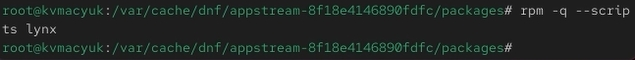
\includegraphics[width=0.7\linewidth,height=\textheight,keepaspectratio]{image/33.jpg}

}

\caption{\label{fig-033}Проверка скриптов установки}

\end{figure}%

Вывод пуст, что означает отсутствие скриптов установки/удаления для
пакета \texttt{lynx}.

В отдельном терминале под своей учётной записью запустил текстовый
браузер \texttt{lynx}, чтобы проверить корректность установки пакета
(рис.~\ref{fig-034}, рис.~\ref{fig-035}).

\begin{figure}

\centering{

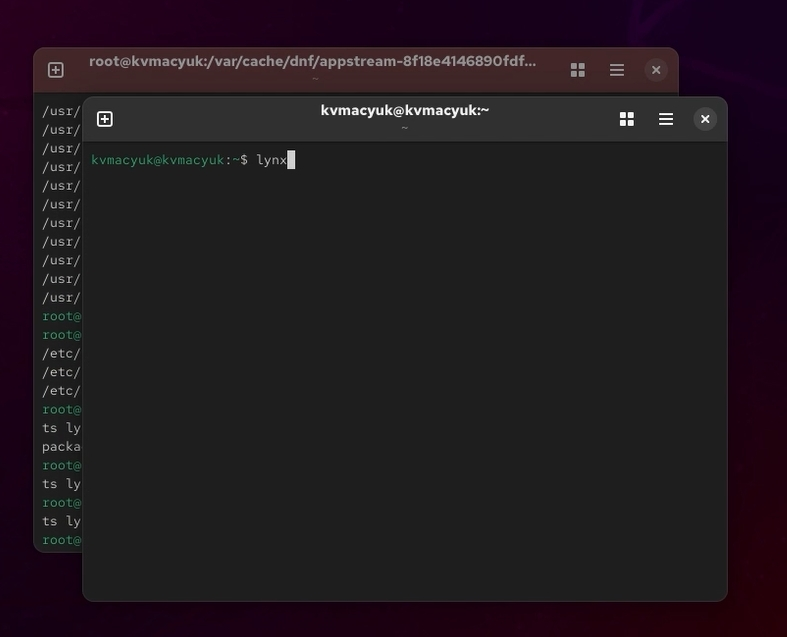
\includegraphics[width=0.7\linewidth,height=\textheight,keepaspectratio]{image/34.jpg}

}

\caption{\label{fig-034}Запуск lynx из-под обычного пользователя}

\end{figure}%

\begin{figure}

\centering{

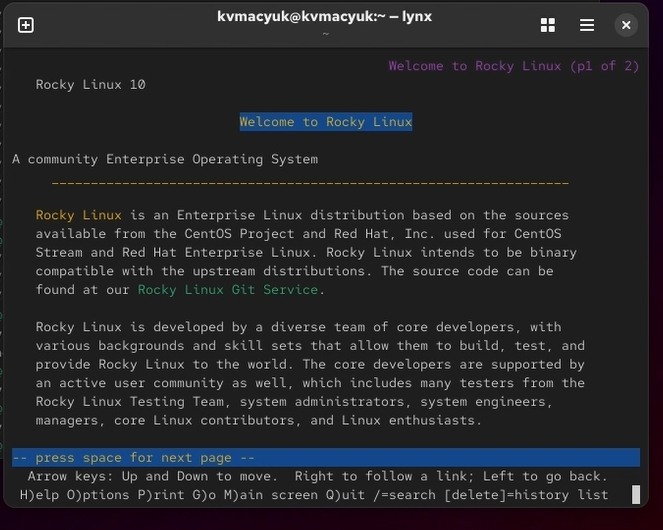
\includegraphics[width=0.7\linewidth,height=\textheight,keepaspectratio]{image/35.jpg}

}

\caption{\label{fig-035}Работа в текстовом браузере}

\end{figure}%

Вернулся в терминал с учётной записью root и удалил пакет
(рис.~\ref{fig-036}).

\begin{Shaded}
\begin{Highlighting}[]
\ExtensionTok{rpm} \AttributeTok{{-}e}\NormalTok{ lynx}
\FunctionTok{ls}
\end{Highlighting}
\end{Shaded}

\begin{figure}

\centering{

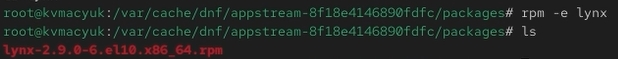
\includegraphics[width=0.7\linewidth,height=\textheight,keepaspectratio]{image/36.jpg}

}

\caption{\label{fig-036}Удаление пакета через rpm}

\end{figure}%

Предположим, что требуется из rpm-пакетов установить \texttt{dnsmasq}
(DNS-, DHCP- и TFTP-сервер).

Установил пакет \texttt{dnsmasq} и определил расположение исполняемого
файла (рис.~\ref{fig-037}---рис.~\ref{fig-039}).

\begin{Shaded}
\begin{Highlighting}[]
\ExtensionTok{dnf}\NormalTok{ list dnsmasq}
\ExtensionTok{dnf}\NormalTok{ install dnsmasq}
\FunctionTok{which}\NormalTok{ dnsmasq}
\end{Highlighting}
\end{Shaded}

\begin{figure}

\centering{

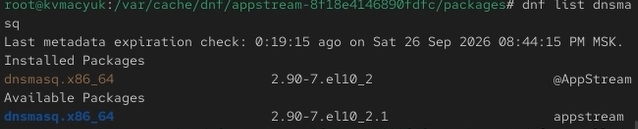
\includegraphics[width=0.7\linewidth,height=\textheight,keepaspectratio]{image/37.jpg}

}

\caption{\label{fig-037}Сравнение версий dnsmasq}

\end{figure}%

\begin{figure}

\centering{

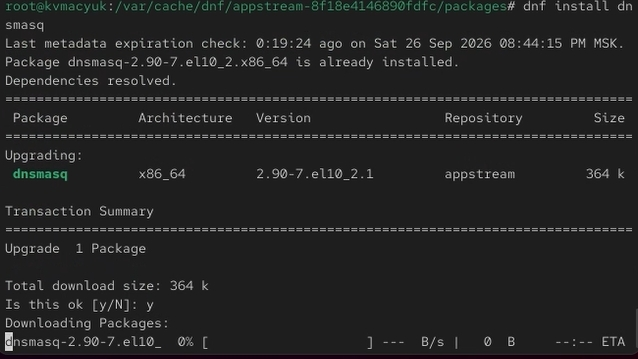
\includegraphics[width=0.7\linewidth,height=\textheight,keepaspectratio]{image/38.jpg}

}

\caption{\label{fig-038}Обновление пакета dnsmasq}

\end{figure}%

\begin{figure}

\centering{

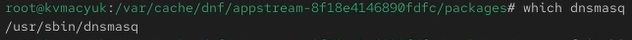
\includegraphics[width=0.7\linewidth,height=\textheight,keepaspectratio]{image/39.jpg}

}

\caption{\label{fig-039}Определение пути dnsmasq}

\end{figure}%

Определил по имени файла, к какому пакету принадлежит \texttt{dnsmasq},
и получил дополнительную информацию о содержимом пакета
(рис.~\ref{fig-040}---рис.~\ref{fig-043}).

\begin{Shaded}
\begin{Highlighting}[]
\ExtensionTok{rpm} \AttributeTok{{-}qf} \VariableTok{$(}\FunctionTok{which}\NormalTok{ dnsmasq}\VariableTok{)}
\ExtensionTok{rpm} \AttributeTok{{-}qi}\NormalTok{ dnsmasq}
\end{Highlighting}
\end{Shaded}

\begin{figure}

\centering{

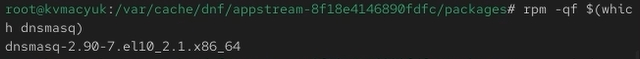
\includegraphics[width=0.7\linewidth,height=\textheight,keepaspectratio]{image/40.jpg}

}

\caption{\label{fig-040}Проверка владельца файла}

\end{figure}%

\begin{figure}

\centering{

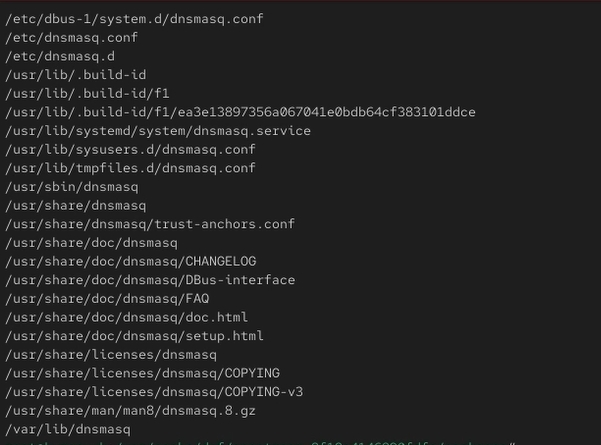
\includegraphics[width=0.7\linewidth,height=\textheight,keepaspectratio]{image/41.jpg}

}

\caption{\label{fig-041}Список файлов пакета dnsmasq}

\end{figure}%

\begin{figure}

\centering{

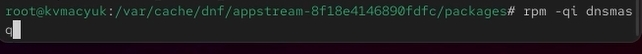
\includegraphics[width=0.7\linewidth,height=\textheight,keepaspectratio]{image/42.jpg}

}

\caption{\label{fig-042}Запрос детальной информации}

\end{figure}%

\begin{figure}

\centering{

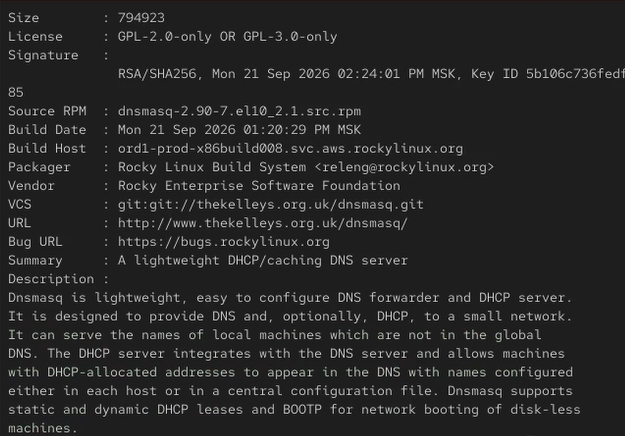
\includegraphics[width=0.7\linewidth,height=\textheight,keepaspectratio]{image/43.jpg}

}

\caption{\label{fig-043}Детальная информация о dnsmasq}

\end{figure}%

Получил список всех файлов в пакете, а также вывел перечень файлов с
документацией пакета (рис.~\ref{fig-044}---рис.~\ref{fig-046}).
Посмотрел файлы документации, применив команду \texttt{man\ dnsmasq}.

\begin{Shaded}
\begin{Highlighting}[]
\ExtensionTok{rpm} \AttributeTok{{-}ql}\NormalTok{ dnsmasq}
\ExtensionTok{rpm} \AttributeTok{{-}qd}\NormalTok{ dnsmasq}
\FunctionTok{man}\NormalTok{ dnsmasq}
\end{Highlighting}
\end{Shaded}

\begin{figure}

\centering{

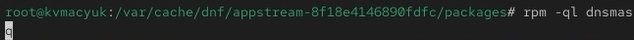
\includegraphics[width=0.7\linewidth,height=\textheight,keepaspectratio]{image/44.jpg}

}

\caption{\label{fig-044}Запрос списка файлов}

\end{figure}%

\begin{figure}

\centering{

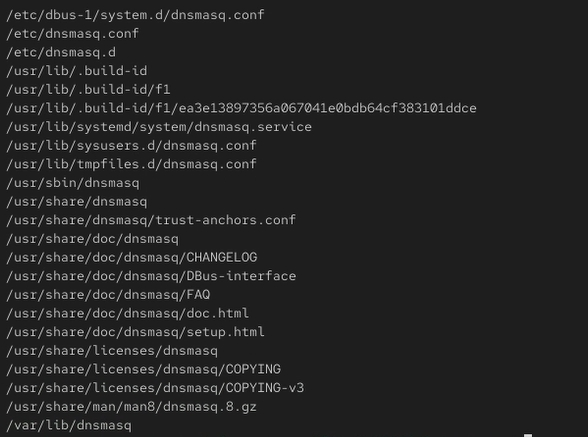
\includegraphics[width=0.7\linewidth,height=\textheight,keepaspectratio]{image/45.jpg}

}

\caption{\label{fig-045}Список файлов (повтор)}

\end{figure}%

\begin{figure}

\centering{

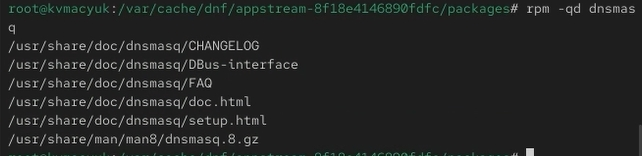
\includegraphics[width=0.7\linewidth,height=\textheight,keepaspectratio]{image/46.jpg}

}

\caption{\label{fig-046}Список документации dnsmasq}

\end{figure}%

\begin{figure}

\centering{

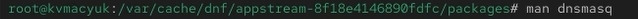
\includegraphics[width=0.7\linewidth,height=\textheight,keepaspectratio]{image/47.jpg}

}

\caption{\label{fig-047}Просмотр man-страницы}

\end{figure}%

Вывел на экран перечень и месторасположение конфигурационных файлов
пакета (рис.~\ref{fig-048}).

\begin{Shaded}
\begin{Highlighting}[]
\ExtensionTok{rpm} \AttributeTok{{-}qc}\NormalTok{ dnsmasq}
\end{Highlighting}
\end{Shaded}

\begin{figure}

\centering{

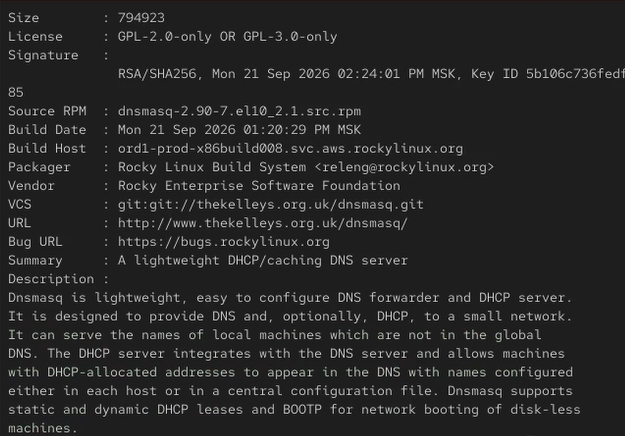
\includegraphics[width=0.7\linewidth,height=\textheight,keepaspectratio]{image/48.jpg}

}

\caption{\label{fig-048}Поиск конфигурационных файлов}

\end{figure}%

Вывел на экран расположение и содержание скриптов, выполняемых при
установке пакета (рис.~\ref{fig-049}).

\begin{Shaded}
\begin{Highlighting}[]
\ExtensionTok{rpm} \AttributeTok{{-}q} \AttributeTok{{-}{-}scripts}\NormalTok{ dnsmasq}
\end{Highlighting}
\end{Shaded}

\begin{figure}

\centering{

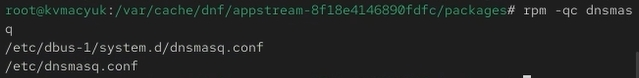
\includegraphics[width=0.7\linewidth,height=\textheight,keepaspectratio]{image/49.jpg}

}

\caption{\label{fig-049}Просмотр скриптов установки}

\end{figure}%

Скрипты предназначены для создания пользователя \texttt{dnsmasq} и
настройки systemd-сервиса при установке, а также для его остановки и
удаления пользователя при удалении пакета.

Вернулся в терминал с учётной записью root и удалил пакет
(рис.~\ref{fig-050}, рис.~\ref{fig-051}).

\begin{Shaded}
\begin{Highlighting}[]
\ExtensionTok{rpm} \AttributeTok{{-}e}\NormalTok{ dnsmasq}
\FunctionTok{ls}
\end{Highlighting}
\end{Shaded}

\begin{figure}

\centering{

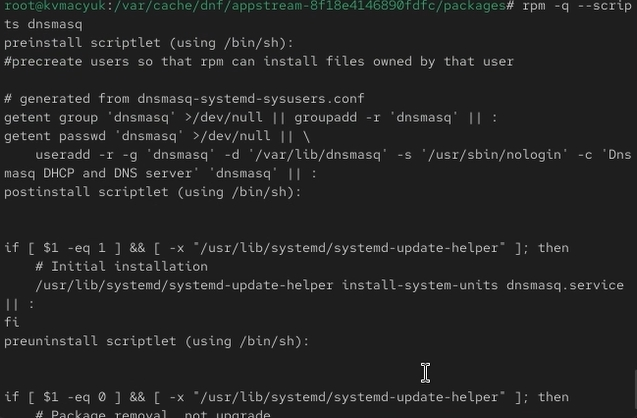
\includegraphics[width=0.7\linewidth,height=\textheight,keepaspectratio]{image/50.jpg}

}

\caption{\label{fig-050}Удаление пакета dnsmasq}

\end{figure}%

\begin{figure}

\centering{

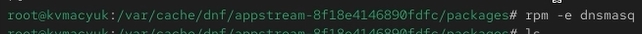
\includegraphics[width=0.7\linewidth,height=\textheight,keepaspectratio]{image/51.jpg}

}

\caption{\label{fig-051}Детальная информация о dnsmasq (повтор)}

\end{figure}%

\chapter{Ответы на контрольные
вопросы}\label{ux43eux442ux432ux435ux442ux44b-ux43dux430-ux43aux43eux43dux442ux440ux43eux43bux44cux43dux44bux435-ux432ux43eux43fux440ux43eux441ux44b}

\textbf{1. Какая команда позволяет вам искать пакет rpm, содержащий файл
useradd?}

Для поиска пакета, содержащего файл \texttt{useradd}, используется
команда \texttt{dnf\ provides\ */useradd} или
\texttt{dnf\ provides\ "*bin/useradd"}. Также можно использовать
\texttt{rpm\ -qf\ \$(which\ useradd)}, если файл уже установлен в
системе.

\textbf{2. Какие команды вам нужно использовать, чтобы показать имя
группы dnf, которая содержит инструменты безопасности и показывает, что
находится в этой группе?}

Для отображения списка групп пакетов используется команда
\texttt{dnf\ grouplist}. Для получения информации о конкретной группе,
содержащей инструменты безопасности (например, «Security Tools»),
используется команда \texttt{dnf\ groupinfo\ "Security\ Tools"}.

\textbf{3. Какая команда позволяет вам установить rpm, который вы
загрузили из Интернета и который не находится в репозиториях?}

Для установки локального rpm-пакета используется команда
\texttt{rpm\ -Uhv\ имя\_пакета.rpm} или
\texttt{dnf\ install\ имя\_пакета.rpm}. Также можно использовать
\texttt{dnf\ install\ http://server/repo/имя\_пакета.rpm} для установки
из сети.

\textbf{4. Вы хотите убедиться, что пакет rpm, который вы загрузили, не
содержит никакого опасного кода сценария. Какая команда позволяет это
сделать?}

Для просмотра скриптов, выполняемых при установке/удалении пакета,
используется команда \texttt{rpm\ -q\ -\/-scripts\ имя\_пакета}. Она
выводит содержимое скриптов, что позволяет проверить их на наличие
опасных действий.

\textbf{5. Какая команда показывает всю документацию в rpm?}

Для отображения списка файлов документации, входящих в пакет,
используется команда \texttt{rpm\ -qd\ имя\_пакета}. Для просмотра всей
документации можно также использовать
\texttt{rpm\ -ql\ имя\_пакета\ \textbar{}\ grep\ -E\ \textquotesingle{}man\textbar{}doc\textbar{}html\textquotesingle{}}.

\textbf{6. Какая команда показывает, какому пакету rpm принадлежит
файл?}

Для определения принадлежности файла к пакету используется команда
\texttt{rpm\ -qf\ путь\_к\_файлу}. Например,
\texttt{rpm\ -qf\ \$(which\ lynx)}.

\chapter{Выводы}\label{ux432ux44bux432ux43eux434ux44b}

В ходе лабораторной работы были получены навыки работы с репозиториями и
менеджерами пакетов \texttt{dnf} и \texttt{rpm}. Изучены основные
команды \texttt{dnf} для поиска, установки, обновления, удаления пакетов
и работы с историей действий. Освоены команды \texttt{rpm} для получения
информации о пакетах, их файлах, документации, конфигурационных файлах и
скриптах установки. Изучено расположение конфигурационных файлов
\texttt{dnf} и репозиториев.

\chapter*{Список
литературы}\label{ux441ux43fux438ux441ux43eux43a-ux43bux438ux442ux435ux440ux430ux442ux443ux440ux44b}
\addcontentsline{toc}{chapter}{Список литературы}

\printbibliography[heading=none]





\end{document}
